%%%%%%%%%%%%%%%%%%%%%%%%%%%%%%%%%%%%%%%%%%%%%%
%%%%%%%%%%%%%%%%%%%%%%%%%%%%%%%%%%%%%%%%%%%%%%
% Cheatsheet Funktionentheorie
% Jens Calov
%%%%%%%%%%%%%%%%%%%%%%%%%%%%%%%%%%%%%%%%%%%%%%
%%%%%%%%%%%%%%%%%%%%%%%%%%%%%%%%%%%%%%%%%%%%%%
\documentclass[
	% Groesse der Standardschrift
	fontsize=7pt,
	% Ausgabeformat
	a4paper,
	% Kein Punkt nach Kapitelnummer
	numbers=noenddot,
]{scrartcl}


% Abstand nach subsection anpassen
\RedeclareSectionCommand[afterskip=0pt]{subsection}


\newcommand{\autor}{Jens Calov}
\newcommand{\titelArbeit}{Funktionentheorie -- Sommersemester 2019}
\title{\titelArbeit}
\author{\autor}
\date{\today}


\usepackage[top=8.5mm,bottom=0mm,left=20mm,right=0mm, twocolumn]{geometry}
\usepackage[utf8]{inputenc}
\usepackage{lmodern}
\usepackage[dvipsnames]{xcolor}
\usepackage[ngerman]{babel}
\usepackage{amssymb}
\usepackage{amsthm}
\usepackage{amsmath}
\usepackage{mathtools}
\usepackage{hyperref}
\usepackage{scrlayer-scrpage}
\usepackage{jgitinfo}
\usepackage{enumitem}
\usepackage{tabto}
\usepackage[framemethod=TikZ]{mdframed}
\usepackage{booktabs}
\usepackage{graphicx}
\usepackage{siunitx}


\setlength{\parindent}{0em}
\addtokomafont{pagenumber}{\sffamily}
\numberwithin{equation}{section}

\makeatletter
\hypersetup{
	colorlinks,
	pdfpagelabels,
	pdfstartview = FitH,
	bookmarksopen = true,
	bookmarksnumbered = true,
	linkcolor = black,
	urlcolor = blue,
	plainpages = false,
	citecolor = black,
	pdftitle = \@title,
	pdfauthor = \@author,
	pdfsubject=\@subject,
	pdfkeywords={\@author, Funktionentheorie, Bachelor, Prof. Dr. Reitz, Bachelor, Hochschule f\"ur Technik Stuttgart, Mathematik}
}
\makeatother

\lohead{\textsf{\autor\ \textsf{\tiny{\textcolor{gray}{Stand: \gitCommitterDate\ $\vert$ Git-Commit: \gitAbbrevHash\ \jgitinfoRelease}}}}}
\cohead{\textsf{Cheatsheet \titelArbeit}}
\rohead{\textsf{Seite \pagemark}}
\lofoot{}
\cofoot{}
\rofoot{}
\KOMAoption{headsepline}{true}
\KOMAoption{footsepline}{false}


\newcommand*{\C}{\mathbb{C}}
\newcommand*{\Co}{\mathbb{C}\setminus\{0\}}
\newcommand*{\Ch}{\hat{\mathbb{C}}}
\newcommand*{\N}{\mathbb{N}}
\newcommand*{\Q}{\mathbb{Q}}
\newcommand*{\R}{\mathbb{R}}
\newcommand*{\Z}{\mathbb{Z}}
\renewcommand*{\Re}{\operatorname{Re}}
\renewcommand*{\Im}{\operatorname{Im}}
\newcommand*{\Ln}{\operatorname{Ln}}
\newcommand*{\argu}{\operatorname{arg}}
\renewcommand{\mod}{\text{mod\,}}

\definecolor{greeny}{rgb}{0,.39,0}
\newcommand{\begriff}[1]{\textcolor{greeny}{\textbf{#1}}}
\newcommand{\VL}[2]{
	\marginpar{\rule{5cm}{0.4pt}}
	\marginpar{\scriptsize{VL#1, #2}}
}

% StyleSkript für Definitionen, Sätze, ...
\newcommand{\jtitlefont}{\sffamily\bfseries}
\newcommand{\jroundedcorner}{5pt}
\newcommand{\jskipabove}{0pt}
\newcommand{\jskipbelow}{-0.73\baselineskip}
\newcommand{\jcolor}{blue!17}



% Satz
\newcounter{satz}[section]
\setcounter{satz}{0}
\newcommand{\satztitel}{Satz~\arabic{section}.\arabic{satz}}
\renewcommand{\thesatz}{\arabic{section}.\arabic{satz}}
\newenvironment{satz}[2][]{
	\refstepcounter{satz}
	\renewcommand{\jcolor}{orange!50}
	\ifstrempty{#1}{
		\mdfsetup{
			frametitle={
				\tikz[baseline=(current bounding box.east),outer sep=0pt]
				\node[anchor=east,rectangle,rounded corners,fill=\jcolor]{\strut \satztitel~\mdseries{(#2)}};
			}
		}
	}{
		\mdfsetup{
			frametitle={
				\tikz[baseline=(current bounding box.east),outer sep=0pt]
				\node[anchor=east,rectangle,rounded corners,fill=\jcolor]{\strut \satztitel:~#1 \mdseries{(#2)}};
			}
		}
	}
	\mdfsetup{
			innertopmargin=-2pt,
			linecolor=\jcolor,
			linewidth=2pt,
			topline=true,
			backgroundcolor=none,
			frametitleaboveskip=\dimexpr-\ht\strutbox\relax,
			frametitlefont=\jtitlefont,
			roundcorner=\jroundedcorner,
			skipabove=\jskipabove,
			skipbelow=\jskipbelow,
	}
	\noindent
	\begin{mdframed}[nobreak=true]\relax
	}{
		\end{mdframed}
}



% Definition
\newcounter{definition}[section]
\setcounter{definition}{0}
\newcommand{\definitiontitel}{Definition~\arabic{section}.\arabic{definition}}
\renewcommand{\thedefinition}{\arabic{section}.\arabic{definition}}
\newenvironment{definition}[2][]{
	\refstepcounter{definition}
	\renewcommand{\jcolor}{yellow!50}
	\ifstrempty{#1}{
		\mdfsetup{
			frametitle={
				\tikz[baseline=(current bounding box.east),outer sep=0pt]
				\node[anchor=east,rectangle,rounded corners,fill=\jcolor]{\definitiontitel~\mdseries{(#2)}};
			}
		}
	}{
		\mdfsetup{
			frametitle={
				\tikz[baseline=(current bounding box.east),outer sep=0pt]
				\node[anchor=east,rectangle,rounded corners,fill=\jcolor]{\definitiontitel:~#1 \mdseries{(#2)}};
			}
		}
	}
	\mdfsetup{
			innertopmargin=-2pt,
			linecolor=\jcolor,
			linewidth=2pt,
			topline=true,
			backgroundcolor=none,
			frametitleaboveskip=\dimexpr-\ht\strutbox\relax,
			frametitlefont=\jtitlefont,
			roundcorner=\jroundedcorner,
			skipabove=\jskipabove,
			skipbelow=\jskipbelow,
	}
	\noindent
	\begin{mdframed}[nobreak=true]\relax
	}{
		\end{mdframed}
}



% Bemerkung
\newenvironment{bemerkung}[2]{
	\renewcommand{\jcolor}{blue!17}
	\mdfsetup{
			frametitle={
				\tikz[baseline=(current bounding box.east),outer sep=0pt]
				\node[anchor=east,rectangle,rounded corners,fill=\jcolor]{#1 \mdseries{(#2)}};
			},
			innertopmargin=-2pt,
			linecolor=\jcolor,
			linewidth=2pt,
			topline=true,
			backgroundcolor=none,
			frametitleaboveskip=\dimexpr-\ht\strutbox\relax,
			frametitlefont=\jtitlefont,
			roundcorner=\jroundedcorner,
			skipabove=\jskipabove,
			skipbelow=\jskipbelow,
	}
	\noindent
	\begin{mdframed}[nobreak=true]\relax
	}{
		\end{mdframed}
}



\begin{document}

	\section{Grundlagen}



\subsection{Komplexe Zahlen}

\begin{bemerkung}{Komplexe Zahlen}{S. 7}
  \begriff{Imaginäre Einheit}:
  \begin{align}
    i^2 = -1
  \end{align}
  Alle Zahlen der Form
  \begin{align}
    z = x + iy, \quad x,y \in \R
  \end{align}
  bilden die Menge
  \begin{align}
    \label{eq:1_2}
    \C \coloneqq \{ z = x + i \cdot y :\ x,y \in \R \}
  \end{align}
  \begriff{Realteil} von $z$:
  \begin{align}
    \operatorname{Re}(z) \coloneqq x \in \R
  \end{align}
  \begriff{Imaginärteil} von $z$:
  \begin{align}
    \operatorname{Im}(z) \coloneqq y \in \R
  \end{align}
\end{bemerkung}

\begin{bemerkung}{Addition}{S. 8}
  Sei $z = x + i \, y \in \C$ und $w = u + i \, v \in \C$.
  \begin{align}
    \label{eq:addition}
    z + w \coloneqq (x + u) + i \, (y + v) \in \C
  \end{align}
\end{bemerkung}

\begin{bemerkung}{Inverses Element bzgl. Addition}{S. 8}
  Sei $z = x + i \, y \in \C$.
  \begin{align}
    \label{eq:inv_addition}
    -z = (-x) + i \, (-y) = - x - i \, y \in \C
  \end{align}
\end{bemerkung}

\begin{bemerkung}{Multiplikation}{S. 8}
  Sei $z = x + i \, y \in \C$ und $w = u + i \, v \in \C$.
  \begin{align}
    \label{eq:multiplikation}
    z \cdot w
      \coloneqq (x + i \, y) \cdot (u + i \, v)
      = (x \, u - y \, v) + i \, (x \, v + y \, u)
      \in \C
  \end{align}
\end{bemerkung}

\begin{bemerkung}{Inverses Element bzgl. Multiplikation}{S. 8}
  Sei $z = x + i \, y \in \C, z \neq 0$.
  \begin{align}
    \label{eq:inv_multiplikation}
    \frac{1}{z}
      &= \frac{1}{(x + i \, y)}
       = \frac{x - i \, y}{(x + i \, y) \, (x - i \, y)}
       % = \frac{x - i \, y}{x^2 - (i \, y)^2}
       = \frac{x - i \, y}{x^2 - i^2 \, y^2}
       = \frac{x - i \, y}{x^2 + y^2}
        \notag\\
      &= \frac{x}{x^2 + y^2} - i \cdot \frac{y}{x^2 + y^2} \in \C
  \end{align}
\end{bemerkung}

\begin{satz}[Körpereigenschaften von $\C$]{S. 8}
  Die Menge $\C$ der komplexen Zahlen bilden mit oben definierter Addition \eqref{eq:addition} bzw. Multiplikation \eqref{eq:multiplikation} einen Körper.
  Das Einselement dieses Körpers ist
  \begin{align}
    1 + 0 \cdot i = 1 \in \C
  \end{align}
  und das Nullelement ist
  \begin{align}
    z = 0 + 0 \cdot i = 0 \in \C .
  \end{align}
  Es gelten somit die Rechenregeln (für $z, v, w \in \C$; $z = x + i \cdot y$):
  \newcommand{\tabone}{39mm}
  \begin{enumerate}[label=\alph*)]
    \item $(z + v) + w = z + (v + w)$ \tabto{\tabone} Assioziativgesetz
    \item $z + 0 = z$ \tabto{\tabone} neutrales Element
    \item $z + (-z) = 0$ \tabto{\tabone} inverses Element; wobei \eqref{eq:inv_addition} gilt
    \item $z + w = w + z$ \tabto{\tabone} Kommutativgesetz
    \item $(z \cdot v) \cdot w = z \cdot (v \cdot v)$ \tabto{\tabone} Assoziativgesetz
    \item $z \cdot 1 = z$ \tabto{\tabone}  neutrales Element
    \item $\displaystyle z \cdot \frac{1}{z} = 1$ für $z \neq 0$ \tabto{\tabone} inverses Element; wobei \eqref{eq:inv_multiplikation} gilt
    \item $z \cdot w = w \cdot z$ \tabto{\tabone} Kommutativgesetz
    \item $z \cdot (v + w) = z \cdot v + z \cdot w$ \tabto{\tabone} Distributivgesetz
  \end{enumerate}
\end{satz}

\begin{bemerkung}{Binomische Formel}{S. 10}
  Mit $z, w \in \C$ und $n \in \N$:
  \begin{align}
    (z + w)^n
      = \sum_{k=0}^n \binom{n}{k} \cdot z^k \cdot w^{n-k}
      = \sum_{k=0}^n \frac{n!}{k! \, (n-k)!} \cdot z^k \cdot w^{n-k}
  \end{align}
\end{bemerkung}

\begin{definition}[Absolutbetrag, konjugiert komplexe Zahl]{S. 10}
  \label{def:absolutbetrag}
  Es sei $z = x + i \cdot y = (x, y) \in \C$.
  Dann ist
  \[ |z| \coloneqq \sqrt{x^2 + y^2} \geq 0 \in \R \]
  der \begriff{Absolutbetrag} von $z$ und
  \[ \overline{z} \coloneqq x - i \cdot y \]
  die zu $z$ \begriff{konjugiert komplexe Zahl}.
\end{definition}

\begin{bemerkung}{Absolutbetrag mit konjugiert komplexer Zahl}{S. 11}
  Wegen $z \cdot \overline{z} = (x + i \, y) \, (x - i \, y) = x^2 - i^2 y^2 = x^2 + y^2 = |z|^2$ folgt:
  \begin{align}
    |z| = \sqrt{z \cdot \overline{z}}
  \end{align}
\end{bemerkung}

\begin{bemerkung}{Abstand komplexer Zahlen}{S. 11}
  Sei $z = x + i \, y \in \C$ und $w = u + i \, v \in \C$.
  Dann ist ihr Abstand:
  \begin{align}
    | z - w |
      = | (x-u) + i \, (y-v) |
      \stackrel{\text{\tiny{Def. \ref{def:absolutbetrag}}}}{=} \sqrt{(x-u)^2 + (y-v)^2 }
  \end{align}
\end{bemerkung}

\begin{satz}[Rechenregeln]{S. 11}
  Für $z = x + i \, y$, $w = u + i \, v$ gelten folgende Rechenregeln:
  \begin{enumerate}
    \item $\displaystyle \overline{z \pm w} = \overline{z} \pm \overline{w}$
    \item $\displaystyle \overline{z \cdot w} = \overline{z} \cdot \overline{w}$
    \item $\displaystyle \overline{\left( \frac{z}{w} \right)} = \frac{\overline{z}}{\overline{w}}$ $(w \neq 0)$
    \item $\displaystyle \overline{\left( \overline{z} \right)} = \overline{z}$
    \item $\displaystyle \left| \overline{z} \right| = \left| z \right|$
    \item $\displaystyle \operatorname{Re}(z) = \frac{z + \overline{z}}{2}$\\
      $\displaystyle \operatorname{Im}(z) = \frac{z - \overline{z}}{2}$
    \item $\displaystyle \operatorname{Re}(z_1 + \dots + z_n) = \operatorname{Re}(z_1) + \dots + \operatorname{Re}(z_n)$\\
      $\displaystyle \operatorname{Im}(z_1 + \dots + z_n) = \operatorname{Im}(z_1) + \dots + \operatorname{Im}(z_n)$
    \item $\displaystyle \operatorname{Re}(z) \leq |z|$\\
      $\displaystyle \operatorname{Im}(z) \leq |z|$
    \item $\displaystyle | z \cdot w | = |z| \cdot |w|$\\
      $\displaystyle \left| \frac{z}{w} \right| = \frac{|z|}{|w|}$ $(w \neq 0)$
  \end{enumerate}
\end{satz}

\begin{bemerkung}{Dreiecksungleichung}{S. 12}
  Sei $z, w \in \C$.
  Dann gilt (wie im Reellen) für den Betrag im Komplexen die \begriff{Dreiecksungleichung}:
  \begin{align}
    | z \pm w | \leq |z| + |w|
  \end{align}
  Allgemein gilt:
  \begin{align}
    \left| \sum_{k=1}^n z_k \right| \leq \sum_{k=1}^n z_k \left| z_k \right|
  \end{align}
\end{bemerkung}

\begin{definition}[Kreisscheibe, $r$-Umgebung einer komplexen Zahl]{S. 12}
  \label{def:1_2}
  Es sei $a \in \C$ und $r \in \R$, $r > 0$.
  Dann ist die Menge
  \begin{align}
    K_r (a) \coloneqq \{ z \in \C : \ |z-a| < r \}
  \end{align}
  die \begriff{(offene) Kreisscheibe} um $a$ mit Radius $r>0$ (oder \begriff{$r$-Umgebung} von $a$)
\end{definition}

\begin{bemerkung}{Polarkoordinatendarstellung komplexer Zahlen}{S. 14}
  Eine komplexe Zahl $z = x + i \, y, z = 0$, ist eindeutig bestimmt durch den \begriff{Betrag}
  \begin{align}
    r \coloneqq |z| = \sqrt{x^2 + y^2}
  \end{align}
  und durch das \begriff{Argument}
  \begin{align}
    \operatorname{arg}(z) \coloneqq \varphi, \ (0 \leq \varphi < 2\pi).
  \end{align}
  Es gilt:
  \begin{align}
    x = |z| \cdot \cos\varphi \text{ und } y = |z| \cdot \sin\varphi .
  \end{align}
  Man nennt
  \begin{align}
    z = r \cdot \left( \cos\varphi + i \cdot \sin\varphi \right)
  \end{align}
  die \begriff{Polarkoordinatendarstellung} von $z \neq 0$.
  Es gilt auch:
  \begin{align}
    z = r \cdot \left[ \cos (\varphi + 2 k \pi) + i \cdot \sin (\varphi + 2 k \pi) \right],\ k \in \Z .
  \end{align}
\end{bemerkung}

\begin{bemerkung}{Umrechnung zwischen Darstellungen}{S. 15}
  Für die Umrechnung zwischen den Darstellungen $z = x + i \, y$ und $z = r \cdot \left( \cos\varphi + i \cdot \sin\varphi \right)$ gelten folgende Regeln:
  \begin{enumerate}
    \item Gegeben sei $z = x + i \, y \neq 0$.
      Mit
      \begin{align}
        r &\coloneqq |z| = \sqrt{x^2 + y^2} \text{ und}\\
        \operatorname{arg}(z) &= \varphi \coloneqq
          \begin{cases}
            \arccos \frac{x}{r} & \text{für } y \geq 0\\
            2 \pi - \arccos \frac{x}{r} & \text{für } y < 0
          \end{cases}
      \end{align}
      gilt
      \begin{align}
        z = r \cdot \left( \cos\varphi + i \cdot \sin\varphi \right) .
      \end{align}
    \item Gegeben sei $z = r \cdot \left( \cos\varphi + i \cdot \sin\varphi \right)$ mit $r > 0$, $\varphi \in [o,2\pi)$.
      Mit
      \begin{align}
        x &\coloneqq r \cdot \cos \varphi \text{ und}\\
        y &\coloneqq r \cdot \sin \varphi
      \end{align}
      gilt
      \begin{align}
        z = x + i \, y .
      \end{align}
  \end{enumerate}
\end{bemerkung}

\begin{satz}{S. 16}
\label{satz:1_3}
  Sind $z, w \in \C\setminus\{0\}$ mit
  \begin{align}
    z = |z| \cdot \left( \cos\varphi + i \cdot \sin\varphi \right), \quad w = |w| \cdot \left( \cos\psi + i \cdot \sin\psi \right),
  \end{align}
  so gilt
  \begin{align}
    z \cdot w &= |z| \cdot |w| \cdot \left[ \cos(\varphi + \psi) + i \cdot \sin(\varphi + \psi) \right],\\
    \frac{z}{w} &= \frac{|z|}{|w|} \cdot \left[ \cos(\varphi - \psi) + i \cdot \sin(\varphi - \psi) \right] .
  \end{align}
\end{satz}

\begin{bemerkung}{Folgerung}{S. 16}
  Aus Satz \ref{satz:1_3} folgt:
  \begin{align}
    \operatorname{arg}(z \cdot w) = \operatorname{arg}(z) + \operatorname{arg}(w) \quad (\mod 2 \pi)\\
    \operatorname{arg}\left(\frac{z}{w}\right) = \operatorname{arg}(z) - \operatorname{arg}(w) \quad (\mod 2 \pi)
  \end{align}
\end{bemerkung}



\subsection{Die komplexe Exponentialfunktion (Teil 1)}

\begin{bemerkung}{Reelle Exponentialfunktion}{S. 17}
  Bekannte reelle Exponentialfunktion ($x, y \in \R$):
  \begin{align}
    e^x &= \sum_{n=0}^\infty \frac{x^n}{n!},\\
    e^{x+y} &= e^x \cdot e^y
  \end{align}
\end{bemerkung}

\begin{bemerkung}{Komplexe Exponentialfunktion}{S. 17}
  Bekannte Komplexe Exponentialfunktion ($z, w \in \C$):
  \begin{align}
    e^z &\coloneqq \sum_{n=0}^\infty \frac{z^n}{n!},\\
    e^{z+w} &= e^z \cdot e^w \label{eq:potenz_komplex}
  \end{align}
\end{bemerkung}

\begin{bemerkung}{Eulersche Gleichung}{S. 18}
  Für $x, y \in \R$ und $z \coloneqq x + i\,y$ gilt:
  \begin{align}
    e^{iy} &= \cos(y) + i \, \sin(y) \qquad \text{Eulersche Gleichung}\\
    e^z &= e^x \cdot e^{i \, y} = e^x \cdot e^{i \, y} = e^x \cdot \left[ \cos(y) + i \, \sin(y) \right]
  \end{align}
\end{bemerkung}

\begin{bemerkung}{Eulersche Identität}{S. 18}
  Aus der Eulerschen Gleichung folgt sofort die Eulersche Identität:
  {
    \Huge
    \begin{align}
      e^{i\pi} + 1 = 0 \notag
    \end{align}
  }
\end{bemerkung}

\begin{satz}{S. 19}
  \label{satz:1_4}
  \begin{enumerate}
    \item Es gilt für $y \in \R$:
      \begin{align}
        \cos y &= \operatorname{Re}\left( e^{iy} \right) = \frac{e^{iy} + e^{-iy}}{2},\\
        \sin y &= \operatorname{Im}\left( e^{iy} \right) = \frac{e^{iy} - e^{-iy}}{2i}
      \end{align}
    \item Jede komplexe Zahl $c \in \C\setminus\{0\}$ lässt sich in der Form
      \begin{align}
        z = r \cdot e^{i\varphi}
      \end{align}
      mit $r = |z|$ und $\varphi = \operatorname{arg}(z)$ schreiben.
    \item Für $z \cdot r \cdot e^{i\varphi}$, $w = s \cdot e^{i\psi}$ gilt:
      \begin{align}
        z \cdot w &= r \cdot s \cdot e^{\varphi + \psi}\\
        \frac{z}{w} &= \frac{r}{s} \cdot e^{\varphi - \psi} \ (w \neq 0).
      \end{align}
  \end{enumerate}
\end{satz}

\begin{satz}[Formel von Moivre]{S. 19}
  \label{satz:1_5}
  Für $n \in \N_0$ gilt:
  \begin{align}
    \left( \cos \varphi + i \, \sin \varphi \right)^n = \cos \left( n \, \varphi \right) + i \, \sin \left( n \, \varphi \right)
  \end{align}
\end{satz}



\subsection{Punktmengen in der komplexen Ebene}

\begin{definition}[Gebiet]{S.20}
  Eine Teilmenge $G \subseteq \C$ heißt \begriff{Gebiet}, wenn $G$ offen und zusammenhängen ist.
\end{definition}

\begin{definition}[einfach zusammenhängend]{S.21}
  Ein Gebiet $G \subseteq \C$ heißt \begriff{einfach zusammenhängend}, wenn das Innere jedes in $G$ verlaufenden geschlossenen Streckenzuges ganz zu $G$ gehört, d.h. wenn $G$ keine Löcher hat.
\end{definition}

\begin{bemerkung}{Randpunkt, Rand von $D$}{S. 21}
  Ist $D \subseteq \C$ eine beliebige Menge, so heißt ein Punkt $z \in \C$ ein \begriff{Randpunkt} von $D$, wenn in jeder $r$-Umgebung (Def. \ref{def:1_2} S. \pageref{def:1_2}) von $z$ sowohl Punkte aus $D$ liegen, als auch Punkte, die nicht zu $D$ gehören.
  Der \begriff{Rand von $D$} ist die Menge aller Randpunkte; er wird mit
  \begin{align}
    \partial D
  \end{align}
  bezeichnet.
\end{bemerkung}

\begin{bemerkung}{abgeschlossen}{S. 22}
  Eine Menge $D \subseteq \C$ heißt \begriff{abgeschlossen}, wenn der Rand von $D$ zu $D$ gehört: $\partial D \subseteq D$.
  Man nennt $\overline{D} \coloneqq D \cup \partial D$ den \begriff{Abschluss} von $D$.
\end{bemerkung}

\begin{bemerkung}{beschränkt, unbeschränkt}{S. 22}
  Eine Menge $D \subseteq \C$ kann beschränkt oder unbeschränkt sein.
  Wir nennen $D$ \begriff{beschränkt}, wenn es eine (hinreichend große) Kreisscheibe $K_r(0)$ gibt, die $D$ umfasst.
  Andernfalls heißt $D$ \begriff{unbeschränkt}.
\end{bemerkung}



\subsection{Zahlenfolgen in der komplexen Ebene}

\begin{definition}[konvergente Folge]{S. 22}
  Man sagt, eine komplexe Zahlenfolge $\left( z_n \right)_{n \geq 0}$ \begriff{konvergiert} gegen den Grenzwert $z \in \C$, und man schreibt
  \begin{align}
    \lim_{n \to \infty} z_n = z \quad \text{ oder } \quad z_n \to z ,
  \end{align}
  wenn es zu jedem $\varepsilon > 0$ einen Index $N(\varepsilon) \in \N_0$ gibt, so dass gilt:
  \begin{align}
    | z_n -z | < \varepsilon \quad \text{ für alle } n \in N(\varepsilon) .
  \end{align}
  Konvergiert die Folge nicht, so nennt man sie \begriff{divergent}.
\end{definition}

\begin{bemerkung}{$z_n\to\infty$}{S. 23}
  Wir schreiben $\displaystyle\lim_{n \to \infty} z_n = \infty$, falls für die \textbf{reelle} Folge $\left( |z_n| \right)$ gilt:\\
  \begin{align}
    \displaystyle\lim_{n \to \infty} |z_n| = +\infty . \notag
  \end{align}
\end{bemerkung}

\begin{bemerkung}{Rechenregeln konvergenter komplexer Folgen}{S. 23}
  Wie bei reellen Folgen ist der Grenzwert einer konvergenten komplexen Folge eindeutig bestimmt und es gelten die bekannten Rechenregeln für $z, w \in \C$:
  \begin{align}
    \begin{rcases}
      \displaystyle \lim_{n \to \infty} z_n = z\\
      \displaystyle \lim_{n \to \infty} w_n = w
    \end{rcases}
    \Rightarrow
    \begin{cases}
      \displaystyle \lim_{n \to \infty} \left( z_n \pm w_n \right) &= z \pm w \\
      \displaystyle \lim_{n \to \infty} \left( z_n \cdot w_n \right) &= z \cdot w \\
      \displaystyle \lim_{n \to \infty} \frac{z_n}{w_n} &= \displaystyle \frac{z}{w} \ (w_n, w \neq 0) \\
      \displaystyle \lim_{n \to \infty} |z_n| &= |z|
    \end{cases}
  \end{align}
\end{bemerkung}

	\section{Elementare Funktionen}

\subsection{Grundlagen}

\subsection{Grenzwerte und Stetigkeit}

\subsection{Die komplexe Exponentialfunktion (Teil 2)}

\subsection{Der komplexe Logarithmus und allgemeine Potenzen}

\subsection{Die trigonometrischen Funktionen}

\subsection{Wurzeln}

\subsection{Möbius-Transformationen}

	\section{Potenzreihen}

\subsection{Unendliche Reihen}

\begin{bemerkung}{Unendliche Reihe}{S. 39}
  Die mit einer komplexen Zahlenfolge $(z_n)_{n \geq 0}$ gebildete Partialsummenfolge
  \begin{align}
    s_n \coloneqq \sum_{k=0}^n z_k = z_0 + z_1 + \cdots + z_n, \quad n \geq 0 ,
  \end{align}
  heißt \begriff{unendliche Reihe}, sie wird mit
  \begin{align}
    \sum_{k=0}^\infty z_k \quad \text{ oder } \quad z_0 + z_1 + z_2 + \cdots
  \end{align}
  bezeichnet.
\end{bemerkung}

\begin{bemerkung}{Konvergenz, Divergenz}{S. 39}
  Man sagt, die Reihe \begriff{konvergiert} gegen $s \in \C$, bzw. sie hat die \begriff{Summe $s \in \C$}, und man schreibt
  \begin{align}
    \sum_{k=0}^\infty z_k = s ,
  \end{align}
  wenn
  \begin{align}
    \lim_{n \to \infty} s_n = \lim_{n \to \infty} (z_0 + z_1 + z_2 + \cdots) = s .
  \end{align}
  Die Reihe (\glqq Summe\grqq) \begriff{divergiert}, wenn sie nicht konvergiert.
\end{bemerkung}

\begin{bemerkung}{Absolute Konvergenz}{S. 39}
  Die Reihe $\displaystyle \sum_{k=0}^\infty z_k = z_0 + z_1 + z_2 + \cdots$ heißt \begriff{absolut konvergent}, wenn die reelle Reihe der Beträge $\displaystyle \sum_{k=0}^\infty |z_k|$ konvergiert.
\end{bemerkung}

\begin{satz}{S. 39}
  Eine absolut konvergente Reihe ist auch konvergent:
  \begin{align}
    \sum_{k=0}^\infty |z_k| \quad \text{konvergiert} \qquad \Rightarrow \qquad \sum_{k=0}^\infty z_k \quad \text{konvergiert.}
  \end{align}
\end{satz}

\begin{satz}[Majorantenkriterium]{S. 40}
  Es gelte $|z_k| \leq b_k$ für $k \in \N_0$. Dann gilt:
  \begin{align}
    \sum_{k=0}^\infty bk \quad \text{konvergent} \qquad \Rightarrow \qquad \sum_{k=0}^\infty z_k \quad \text{absolut konvergent.}
  \end{align}
\end{satz}

\begin{satz}[Quotientenkriterium]{S. 40}
  Es gelte $z_k \neq 0$ für $k \geq k_0$. Dann folgt:
  \begin{enumerate}[label=\alph*)]
    \item $\displaystyle \lim_{k \to \infty} \left| \frac{z_{k+1}}{z_k} \right| < 1 \qquad \Rightarrow \qquad \sum_{k=0}^\infty z_k \quad$ absolut konvergent,
    \item $\displaystyle \lim_{k \to \infty} \left| \frac{z_{k+1}}{z_k} \right| > 1 \qquad \Rightarrow \qquad \sum_{k=0}^\infty z_k \quad$ divergent.
  \end{enumerate}
\end{satz}

\begin{bemerkung}{Geometrische Reihe}{S. 40}
  Wie im Reellen gilt für $q \in \C$ mit $|q| < 1$:
  \begin{align}
    \sum_{k=0}^n q^k = \frac{1 - q^{n+1}}{1-q}
  \end{align}
  und damit
  \begin{align}
    \sum_{k=0}^\infty q^k = \frac{1}{1-q}
  \end{align}
\end{bemerkung}



\pagebreak
\subsection{Potenzreihen}

\begin{bemerkung}{Potenzreihe}{S. 40}
  Eine Reihe der Form
  \begin{align}
    \sum_{k=0}^\infty a_k \cdot (z-z_0)^k \label{eq:potenzreihe}
  \end{align}
  mit $a_k, z_0, z \in \C$ heißt \begriff{Potenzreihe} mit \begriff{Zentrum $z_0$} oder \begriff{Entwicklungspunkt $z_0$} und \begriff{Koeffizienten $a_k$}.\\
  \ \\
  \textbf{Achtung}: Es dürfen nur nichtnegative Potenzen von $z - z_0$ auftreten!
\end{bemerkung}

\begin{bemerkung}{Konvergenzrdius}{S. 40}
  Wie im Reellen zeigt man, dass für eine Potenzreihe \eqref{eq:potenzreihe} nur die folgenden drei Fälle auftreten:
  \begin{enumerate}
    % \item $\displaystyle \sum_{k=0}^\infty a_k \, (z-z_0)^k$ konvergiert absolut für alle $z \in \C$.
    % \item $\displaystyle \sum_{k=0}^\infty a_k \, (z-z_0)^k$ konvergiert nur für $z = z_0$.
    % \item Es gibt eine positive Zahl $R$, so dass $\displaystyle \sum_{k=0}^\infty a_k \, (z-z_0)^k$ für alle $z$ mit $|z - z_0| < R$ absolut konvergiert und für $|z - z_0| > R$ divergiert.
    %   Für $|z - z_0| = R$ kann Konvergenz oder Divergenz vorliegen.
    \item Die Potenzreihe konvergiert absolut für alle $z \in \C$.
    \item Die Potenzreihe konvergiert nur für $z = z_0$.
    \item Es gibt eine positive Zahl $R$, so dass die Potenzreihe für alle $z$ mit
      \begin{itemize}
        \item $|z - z_0| < R$ absolut konvergiert,
        \item $|z - z_0| > R$ divergiert,
        \item $|z - z_0| = R$ konvergiert oder divergiert (auch gemischt möglich).
      \end{itemize}
  \end{enumerate}
  Die Zahl $R$ heißt \begriff{Konvergenzradius} der Reihe und $\{ z \in \C : \ |z - z_0| = R \}$ der \begriff{Konvergenzkreis}.
  Zur Vermeidung von Fallunterscheidungen definiert man im Fall 1 den Konvergenzradius $R = \infty$ und im Fall 2 den Konvergenzradius $R = 0$.
\end{bemerkung}

\begin{bemerkung}{Berechnung Konvergenzrdius}{S. 41}
  Zur Berechnung des Konvergenzradius $R$ ist häufig das Quotienten oder Wurzelkriterium anwendbar:
  \begin{align}
    R &= \lim_{k \to \infty} \left| \frac{a_k}{a_{k+1}} \right| \in [0, \infty],\label{eq:R1}\\
    R &= \frac{1}{\displaystyle \limsup_{k \to \infty} \sqrt[k]{\left| a_k \right|}} \in [0, \infty].\label{eq:R2}
  \end{align}
  Der Grenzwert \eqref{eq:R1} existiert nicht immer.
  Der größte Häufungswert \eqref{eq:R2} einer Folge existiert jedoch immer.
\end{bemerkung}



\subsection{Gleichmäßige Konvergenz}

\begin{bemerkung}{Gleichmäßige Konvergenz}{S. 42}
  $\left( f_n(z) \right)$ konvergiert auf $D \subseteq \C$ \begriff{gleichmäßig} gegen die \begriff{Grenzfunktion} $f(z)$, wenn es zu jedem beliebig kleinen Radius $\varepsilon > 0$ einen für alle $z \in D$ gemeinsamen Index $N(\varepsilon)$ gibt, so dass für $n \geq N(\varepsilon)$ sämtliche Funktionswerte $f_n(z)$ in die $\varepsilon$-Umgebung von $f(z)$ fallen:
  \begin{align}
    \left| f_n(z) - f(z) \right| \leq \varepsilon \quad \text{ für alle } z \in D,\ n \geq N(\varepsilon) .
  \end{align}
\end{bemerkung}

\begin{bemerkung}{Punktweise Konvergenz}{S. 42}
  Bei \begriff{punktweiser Konvergenz} ist die \glqq Konvergenzgeschwindigkeit\grqq\ evtl. von Punkt zu Punkt verschieden.
  Bei punktweiser Konvergenz gilt:
  \begin{align}
    \left| f_n(z) - f(z) \right| \leq \varepsilon \quad \text{ für alle } z \in D,\ n \geq N(\varepsilon, \textcolor{blue}{z}) .
  \end{align}
\end{bemerkung}

\begin{bemerkung}{Sätzle: Gleichmäßige Konvergenz einer Potenzreihe}{S. 42}
  Eine Potenzreihe \eqref{eq:potenzreihe} mit Konvergenzradius $R > 0$ ist in jeder abgeschlossenen Kreisscheibe $D$ innerhalb ihres Konvergenzkreises ($D \coloneqq \{ z:\ \left| z - z_0 \right| \leq r < R \}$) gleichmäßig konvergent.
\end{bemerkung}

\begin{bemerkung}{Eigenschaften bei gleichmäßiger Konvergenz einer Potenzreihe}{S. 42}
  Für $\displaystyle s_n(z) \coloneqq \sum_{k=0}^\infty a_k \, (z - z_0)^k$ und $\displaystyle s(z) \coloneqq \sum_{k=0}^\infty a_k \, (z - z_0)^k$ gilt:
  \begin{align}
    \left| s_n(z) - s(z) \right| \leq \varepsilon \quad \text{ für alle } z \in D,\ n \geq N(\varepsilon) .
  \end{align}
  Gleichmäßige Konvergenz garantiert die Eigenschaften der \begriff{Grenzfunktion}:
  \begin{align}
    s(z) \coloneqq \sum_{k=0}^\infty a_k \, (z - z_0)^k , \quad | z - z_0 | < R .
  \end{align}
  Insbesondere ist deshalb $s(z)$ in der Menge $\{ z:\ | z - z_0 | < R \}$ \begriff{stetig}.
  Die Stetigkeit einer Potenzreihe in $z^*$ können wir auch wie folgt schreiben:
  \begin{align}
    \lim_{z \to z^*} s(z) = s(z) = \sum_{n=0}^\infty a_n \, (z^* - z_0)^n .
  \end{align}
  Alle komplexen Funktionen, die über Potenzreihen definiert sind, sind stetig.
\end{bemerkung}

	\section{Differentiation, analytische Funktionen}



\subsection{Definition und Rechenregeln}

\begin{definition}{S. 43}
  Sei $G \subseteq \C$ ein Gebiet und $f:\ G \to \C$.
  $f$ heißt in $z_0 \in G$ \begriff{komplex differenzierbar}, wenn der Grenzwert
  \begin{align}
    \frac{df}{dz} (z_0) \coloneqq f'(z_0) \coloneqq \lim_{z \to z_0} \frac{f(z) - f(z_0)}{z - z_0}
  \end{align}
  im Sinne von Definition \ref{def:2_1} existiert.
  $f'(z_0)$ heißt \begriff{Ableitung} von $f$ an der Stelle $z_0$.
  $f:\ g \to \C$ heißt \begriff{analytisch} (oder \begriff{holomorph}), wenn $f'(z)$ für jedes $z \in G$ existiert.
\end{definition}

\begin{bemerkung}{Bemerkungen, Rechenregeln}{S. 43}
  \begin{enumerate}
    \item Der Grenzwert des Differenzenquotienten muss bei jeder Annäherung von $z$ an $z_0$ existieren und gleich $f'(z_0)$ sein.
      Andernfalls ist die Funktion an $z_0$ nicht differenzierbar.
    \item Differenzierbare Funktionen sind stetig.
    \item Sind $f$ und $g$ differenzierbar (bzw. analytisch), so sind auch die Funktionen $f \pm g$, $f \cdot g$, $\displaystyle \frac{f}{g}$ (für $g(z) \neq 0$) und $f \circ g$ differenzierbar (bzw. analytisch), und es gelten die folgenden Rechenregeln:
    \begin{enumerate}
      \item Linearität:
        \begin{align}
          \left( a \, f + b \, g\right)' = a \, f' + b \, g'
        \end{align}
      \item Produktregel:
        \begin{align}
          \left( f \cdot g\right)' = f' \cdot g + f \cdot g'
        \end{align}
      \item Quotientenregel:
        \begin{align}
          \left( \frac{f}{g} \right)' = \frac{f' \cdot g - f \cdot g'}{g^2}
          \intertext{insbesondere}
          \left( \frac{1}{g} \right)' = - \frac{g'}{g^2}
        \end{align}
      \item Kettenregel:
        \begin{align}
          \big( f \left( g \right) \big)' = f'(g) \cdot g'
        \end{align}
    \end{enumerate}
  \end{enumerate}
\end{bemerkung}

\begin{satz}[Potenzreihen sind analytisch und unendlich oft diff.bar]{S. 45}
  Eine Potenzreihe $\displaystyle f(z) = \sum_{k=0}^\infty a_k \, (z - z_0)^k$ mit Konvergenzradius $R > 0$ stellt im Inneren des Konvergenzkreises eine analytische Funktion dar.
  \begin{align}
    f(z) = \sum_{k=0}^\infty a_k \, (z - z_0)^k
  \end{align}
  ist analytisch in $K_R (z_0) = \{ z: \ |z - z_0| < R \}$.
  Die Ableitung erhält man durch gliedweise Differentiation:
  \begin{align}
    f'(z) = \sum_{\textcolor{blue}{k=1}}^\infty k \, a_k \, (z - z_0)^{k-1}
  \end{align}
  Die abgeleitete Reihe ist wieder eine Potenzreihe und hat denselben Konvergenzradius $R$.
  Das Ableiten kann also beliebig oft wiederholt werden.
  Die Koeffizienten lassen sich aus der Funktion $f$ berechnen und sind daher durch $f$ eindeutig bestimmt:
  \begin{align}
    a_n = \frac{1}{n!} f^{(n)}(z_0), \quad n = 0, 1, 2, \dots\ .
  \end{align}
\end{satz}



\subsection{Die Cauchy-Riemann-Differentialgleichungen}

\begin{satz}[Cauchy-Riemann-Differentialgleichungen]{S. 47}
  \label{satz:4_2}
  Ist $f : \C \to \C$ differenzierbar an $z_0 = x_0 + i \, y_0$ und gilt
  \begin{align}
    f(z) = f(x,y) = u(x,y) + i \, v(x, y) ,
  \end{align}
  so erfüllen $u$ und $v$ die \begriff{Cauchy-Riemann-Differentialgleichungen} an der Stelle $(x_0, y_0)$:
  \begin{align}
    u_x(x_0, y_0) &=   v_y(x_0, y_0) ,\\
    u_y(x_0, y_0) &= - v_x(x_0, y_0) .
  \end{align}
  Ist $f$ differenzierbar für alle $z \in G$, wobei $G$ eine offene Menge in $\C$ ist, so gelten diese Differentialgleichungen in ganz $G$.
\end{satz}

\begin{bemerkung}{Folgerung aus Satz \ref{satz:4_2}: Funktionen mit Ableitung $0$ sind konstant}{S. 47}
  Es sei $f : G \to \C$ ein in dem Gebiet $G \subseteq \C$ analytische Funktion mit $f'(z) = 0$ für alle $z \in G$.
  Dann gilt: $f(z) =$ const.
\end{bemerkung}



\pagebreak
\subsection{Geometrische Deutung der Ableitung}

\begin{satz}{S. 47}
  Ist $f : G \to \C$ eine analytische Funktion mit $f'(z) \neq 0$ in dem Gebiet $G$, dann ist die Abbildung $f : G \to \C$ in allen Punkten $z_0 \in G$ \begriff{lokal konform} (d.h. \begriff{winkeltreu} und \begriff{orientierungstreu}), d.h. der Schnittwinkel zwischen zwei glatten Kurven durch $z_0 \in G$ ist samt Drehsinn der gleiche wie für die beiden Bildkurven durch $f(z_0)$.
\end{satz}



\subsection{Das komplexe Potenzial}





\subsection{Harmonische Funktionen}

\begin{bemerkung}{Harmonische Funktionen}{S. 50}
  Ist $f(z) = u(x,y) + i \, v(x,y)$ eine analytische Funktion, so gilt aufgrund der Cauchy-Riemann-Differentialgleichungen
  \begin{align}
    u_x &= v_y\\
    u_y &= - v_x .
  \end{align}
  Es folgt $u_{xx} = v_{yx}$ und $u_{yy} = -v_{xy}$.
  Wegen $v_{xy} = v_{yx}$ haben wir: $u_{xx} + u_{yy} = 0$.
  Man schreibt dafür auch
  \begin{align}
    \Delta u &= u_{xx} + u_{yy} = 0
  \end{align}
  und nennt Funktionen dieser Eigenschaft \begriff{harmonisch}.
  Es gilt auch
  \begin{align}
    \Delta v &= v_{xx} + v_{yy} = 0 .
  \end{align}
\end{bemerkung}

\begin{bemerkung}{}{S. 50}
  Es sei nun $G \subseteq \C$ einfach zusammenhängend und es sei nur die Funktion $u(x,y)$ vorgegeben.
  Gesucht ist die Funktion $v(x,y)$, sodass
  \begin{align}
    f(z) = u(x,y) + i \, v(x,y) \label{eq:harm_ana}
  \end{align}
  eine analytische Funktion ist.
  Wir gehen wie folgt vor:
  \begin{enumerate}
    \item $u_x$ und $u_y$ berechnen
    \item Aus dem Ansatz $v_y = u_x$ durch unbestimmte Integration nach $y$
      \begin{align}
      v = \int u_x \, dy + c(x)
      \end{align}
      bestimmen.
    \item Nach $x$ differenzieren, $\displaystyle v_x = \frac{\partial}{\partial x} \left( \int u_x \, dy \right) + c'(x)$, dies mit $-u_y$ gleichsetzen und daraus $c(x)$ berechnen.
    \item Zur analytischen Funktion \eqref{eq:harm_ana} zusammensetzen.
  \end{enumerate}
\end{bemerkung}

	\section{Integration}

\subsection{Grundlagen}

\subsection{Der Cauchy-Integralsatz}

\subsection{Die Cauchy-Integralformel}

	\section{Anwendungen der Cauchy-Integralformel}



\subsection{Die Taylor-Reihe}

\begin{satz}{S. 61}
  Es sei $a \in \C$ und $w \neq a$.
  Dann gilt
  \begin{align}
    |w - a| > |z - a| \quad & \Rightarrow &\frac{1}{w-z} = \sum_{k=0}^\infty \frac{(z-a)^k}{(w-a)^{k+1}} , \\
    && (\text{Potenzreihe bzgl. } z) \notag \\
    |w - a| < |z - a| \quad & \Rightarrow &\frac{1}{w-z} = - \sum_{k=0}^\infty \frac{(w-a)^k}{(z-a)^{k+1}} . \\
    && (\text{keine Potenzreihe bzgl. } z) \notag
  \end{align}
\end{satz}

\begin{bemerkung}{Bemerkung}{S. 61}
  Eine analytische Funktion $f$ ist beliebig oft differenzierbar und (lokal) immer durch eine Taylor-Reihe darstellbar.
\end{bemerkung}

\begin{satz}[Taylor-Reihe]{S. 62}
  \label{satz:6_2}
  Jede im Gebiet $G$ analytische Funktion $f$ besitzt innerhalb jeder $r$-Um\-ge\-bung $K_r(a)$ (vgl. Def. \ref{def:1_2}, S. \pageref{def:1_2}), die ganz in $G$ liegt, die Potenzreihendarstelleng (\begriff{Taylor-Entwicklung})
  \begin{align}
    f(z) = \sum_{k=0}^\infty \frac{f^{(k)}(a)}{k!} \, (z - a)^k, \qquad z \in K_r(a);
  \end{align}
  insbesondere ist $f$ in $G$ beliebig oft differenzierbar mit den Ableitungen (\begriff{verallgemeinerte Cauchy-Integralformeln})
  \begin{align}
    f^{(n)}(z) =  \frac{n!}{2 \pi i} \oint_{|w-a|=\rho} \frac{f(w)}{(w-z)^{n+1}} \, dw, \qquad |w-a| < \rho < r, n \in \N_0 .
  \end{align}
\end{satz}

\begin{bemerkung}{Folgerung}{S. 62}
  Ist $f$ in ganz $\C$ analytisch (also $G = \C$), so hat die Taylor-Reihe den Konvergenzradius $R = \infty$.
\end{bemerkung}

\begin{bemerkung}{Regel von l'Hospital}{S. 63}
  Sind $f$ und $g$ analytische Funktionen mit $f(z_0) = g(z_0) = 0$ und gilt $g'(z_0) \neq 0$, so folgt
  \begin{align}
    \lim_{z \to z_0} \frac{f(z)}{g(z)} = \frac{f'(z_0)}{g(z_0)} .
  \end{align}
\end{bemerkung}

\begin{bemerkung}{Bemerkung}{S. 63}
  Ist $R$ der Konvergenzradius der Taylor-Reihe von $f$, so befindet sich auf dem Rand des Konvergenzkreises immer eine Stelle, an der $f$ nicht differenzierbar ist (\glqq Singularität\grqq).
  Für die Funktion $\Ln(1+z)$ ist diese Singularität bei $-1$.
\end{bemerkung}

\begin{definition}{S. 64}
  \label{def:6_1}
  Man sagt, eine analytische Funktion habe eine Nullstelle $a$ der \begriff{Ordnung} $m$, wenn gilt
  \begin{align}
    f(z) = (z - a)^m \cdot f_1(z) \quad \text{in einer Umgebung } K_r(a)
  \end{align}
  mit einer analytischen Funktion $f_1$, für die gilt $f_1(a) \neq 0$.
  Dies ist gleichbedeutend mit
  \begin{align}
    f(a) = f'(a) = \cdots = f^{(m-1)}(a) = 0, \quad f^{(m)}(a) \neq 0 .
  \end{align}
\end{definition}

\begin{satz}[Identitätssatz]{S. 64}
  \label{satz:6_3}
  Für analytische Funktionen $f, g: G \to \C$ auf einem Gebiet $G$ sind äquivalent:
  \begin{enumerate}[label=\alph*)]
    \item $f(z) = g(z)$ für alle $z \in G$
    \item $f(z_n) = g(z_n)$ für alle Punkte $(z_n)$ einer unendlichen Folge mit verschiedenen Folgengliedern und Häufungswert $a$ in $G$.
  \end{enumerate}
\end{satz}



\subsection{Der Fundamentalsatz der Algebra}

\begin{satz}[Satz von Liouville]{S. 65}
  \label{satz:6_4}
  Ist $f$ auf ganz $\C$ analytisch und beschränkt ($|f(z)| \leq M$ für alle $z \in \C$), so ist $f$ eine konstante Funktion: $f(z) =$ const.
\end{satz}

\begin{satz}[Fundamentalsatz der Algebra]{S. 66}
  Jedes nichtkonstante Polynom
  \begin{align}
    p(z) = a_m \, z^n + \cdots + a_1 \, z + a_0, \quad n \geq 1, a_n \neq 0
  \end{align}
  hat in $\C$ genau $n$ Nullstellen, wobei wir eine Nullstelle der Ordnung $m$ (vgl. Def. \ref{def:6_1}) $m$-mal zählen.
\end{satz}



\subsection{Mittelwerteigenschaft und Maximumprinzip}

\begin{bemerkung}{Mittelwerteigenschaft}{S. 66}
  Ist $f: G \to \C$ analytisch, $G$ ein Gebiet, so gilt gemäß Cauchy-Integralformel (Satz \ref{satz:cauchy_integralformel}):
  \begin{align}
    f(z) = \frac{1}{2 \pi i} \oint_{|w-z|=\rho} \frac{f(w)}{w-z} \, dw .
  \end{align}
  Schreiben wir den Kreis $|w-z|=\rho$ in der Form $C = \{ w : w = z + \rho \, e^{it}, \ t \in [0, 2 \pi) \}$, so folgt:
  \begin{align}
    f(z) &= \frac{1}{2 \pi i} \int_0^{2 \pi} \frac{f \left( z + \rho \, e^{it} \right)}{z + \rho \, e^{it}-z} \cdot i \cdot \rho \, e^{it} \, dw \\
    &= \frac{1}{2 \pi} \int_0^{2 \pi} f \left( z + \rho \, e^{it} \right) \, dt
  \end{align}
  Der Funktionswert $f(z)$ ist der mittlere Wert aller Funktionswerte\linebreak
  $f \left( z + \rho \, e^{it} \right)$ auf der Kreislinie $C$ (\begriff{Mittelwerteigenschaft}).
\end{bemerkung}

\begin{satz}[Maximumprinzip]{S. 67}
\label{satz:6_6}
  Ist $G$ ein beschränktes Gebiet, $f: G \cup \partial G \to \C$ analytisch und nicht konstant, dann liegt jede Maximalstelle $z_0$ der Funktion $|f(z)|$ auf dem Rand von $G$ (und nicht im Innern von $G$), d.h. die Betragsfläche $z \to |f(z)|$ hat keine Gipfel im Innern des Gebiets.
\end{satz}



\subsection{Folgen analytischer Funktionen}

\begin{lemma}{S. 68}
  Es sei $f: G \to \C$ stetig, und für jede im Gebiet $G$ verlaufende einfach geschlossene (stückweise stetig differenzierbare) Kurve $C$, sie samt ihres Innern in $G$ liegt, gelte $\oint_C f(z) \, dz = 0$.
  Dann ist $f$ analytisch in $G$.
\end{lemma}

\begin{satz}[Weierstraß]{S. 68}
  \label{satz:6_7}
  Ist $(f_n)$ eine gleichmäßig konvergente Folge analytischer Funktionen in dem Gebiet $G$, so ist auch die Grenzfunktion $f$ analytisch in $G$.
  Es gilt dann
  \begin{align}
    \lim_{n \to \infty} f_n'(z) = f'(z) .
  \end{align}
\end{satz}

\begin{satz}{S. 69}
  \label{satz:6_8}
  Ist $(f_n)$ eine gleichmäßig konvergente Folge analytischer Funktionen mit Grenzfunktion $f$ in dem Gebiet $G$, so gilt
  \begin{align}
    \lim_{n \to \infty} \int_C f_n(z) \, dz = \int_C f(z) \, dz \qquad (n \to \infty)
  \end{align}
  für jede stückweise differenzierbare Kurve $C$ in $G$.
\end{satz}

\begin{bemerkung}{Bemerkung}{S. 69}
  Da in Satz \ref{satz:6_8} $f(z) = \lim_{n \to \infty} f_n(z)$ gilt, können wir auch schreiben:
  \begin{align}
    \lim_{n \to \infty} \int_C f_n(z) \, dz = \int_C \lim_{n \to \infty} f_n(z) \, dz ,
  \end{align}
  falls die Funktionenfolge gleichmäßig konvergiert.
\end{bemerkung}



\subsection{Eigenschaften analytischer Funktionen (Zusammenfassung)}

\begin{bemerkung}{Eigenschaften analytischer Funktionen}{S. 70}
  Es sei $f: G \to \C$ analytisch, $G$ ein einfach zusammenhängendes Gebiet in $\C$ und $C$ eine einfach geschlossene Kurve in $G$.
  Dann gilt:
  \begin{enumerate}
    \item \textbf{Cauchy-Integralsatz} (Satz \ref{satz:cauchy_integralsatz}):
      \begin{align}
        \oint_C f(z) \, dz = 0 .
      \end{align}
    \item $\displaystyle F(z) \coloneqq \int_{z_0}^z f(w) \, dw$ ist wegunabhängig (Satz \ref{satz:5_3}); $F'(z) = f(z)$.
    \item \textbf{Cauchy-Integralformeln} (Sätze \ref{satz:cauchy_integralformel}, \ref{satz:6_2}):
      \begin{align}
        f^{(n)}(z) =  \frac{n!}{2 \pi i} \oint_{C} \frac{f(w)}{(w-z)^{n+1}} \, dw, \qquad n \in \N_0
      \end{align}
      für alle $z$ aus dem Inneren von $C$.
    \item \textbf{Taylor-Entwicklung um $a \in G$} (Satz \ref{satz:6_2}):
      \begin{align}
        f(z) = \sum_{n=0}^\infty \frac{f^{(n)}(a)}{n!} \, (z - a)^n %, \qquad z \in K_r(a);
      \end{align}
      in jeder offenen Kreisscheibe $|z-a| < r$, die ganz in $G$ liegt.
    \item Im Fall $G = \C$ gilt der \textbf{Satz von Liouville} (Satz \ref{satz:6_4}) für beschränkte, analytische Funktionen.
    \item \textbf{Identitätssatz} (Satz \ref{satz:6_3})
    \item \textbf{Mittelwerteigenschaft}:
      \begin{align}
        f(z) = \frac{1}{2 \pi} \int_0^{2 \pi} f \left( z + \rho \, e^{it} \right) \, dt \qquad z \in G .
      \end{align}
    \item \textbf{Maximumprinzip} (Satz \ref{satz:6_6}): Ist $f$ nicht konstant, so nimmt $|f|$ das Maximum auf $\partial G$ an (falls $G$ beschränkt).
    \item \textbf{Konvergenzsätze} (Sätze \ref{satz:6_7}, \ref{satz:6_8}): Ist $(f_n)$ eine gleichmäßig gegen $f$ konvergierende Folge analytische Funktionen, so konvergieren auch die ersten Ableitungen und die Kurvenintegrale der Funktionen $f_n$ gegen die erste Ableitung bzw. das Kurvenintegral von $f$.
  \end{enumerate}
\end{bemerkung}

	\section{Laurent-Reihen und Singularitäten}


\subsection{Laurent-Reihen}

\begin{satz}[Laurent-Reihen]{S. 72}
  \label{satz:7_1}
  Es sei $f$ im Kreisring $K_{r,R}(a) = \{ z : 0 \leq r < |z-a| < R \}$ analytisch, wobei $0 \leq r < r \leq \infty$.
  Dann gilt:
  \begin{enumerate}[label=\alph*)]
    \item $f(z)$ lässt sich für alle $z \in K_{r,R}(a)$ als \begriff{Laurent-Reihe} schreiben:
  \end{enumerate}
  \vspace{-1em}
  \begin{align}
    f(z)
      &= \sum_{n=-\infty}^{\infty} c_n \cdot (z-a)^n
       \coloneqq \sum_{n=0}^{\infty} c_n \cdot (z-a)^n + \sum_{n=1}^{\infty} \frac{c_{-n}}{(z-a)^n}
       \notag\\
      &= \cdots
        + \frac{c_{-2}}{(z-a)^2}
        + \frac{c_{-1}}{z-a}
        + c_0
        + c_1 (z-a)
        + c_2 (z-a)^2
        + \cdots
        .
  \end{align}
  \begin{enumerate}[label=\alph*)]
    \item[b)] Die Koeffizienten $c_n$ sind eindeutig bestimmt durch ($n \in \Z$, $r < \rho < R$):
      \begin{align}
        \label{eq:koeff_c_n}
        c_n = \frac{1}{2 \pi i} \oint_{|w-a| = \rho} \frac{f(w)}{(w-a)^{n+1}} \, dw .
      \end{align}
  \end{enumerate}
\end{satz}

% \begin{bemerkung}{Bemerkungen}{S. 72}
%
% \end{bemerkung}



\subsection{Isolierte Singularitäten}

\begin{bemerkung}{Isolierte Singularität, Hauptteil, Nebenteil}{S. 75}
  Man nennt eine Singularität von $f$ \begriff{isoliert}, wenn $f$ an $z_0$ nicht definiert ist, aber in $\{ z : 0 < |z-z_0| < r \}$ analytisch ist.
  Nach Satz \ref{satz:7_1} besitzt $f$ die Laurent-Entwicklung
  \begin{align}
    f(z)
     &= \cdots
       + \frac{c_{-2}}{(z-z_0)^2}
       + \frac{c_{-1}}{z-z_0}
       + c_0
       + c_1 (z-z_0)
       + c_2 (z-z_0)^2
       + \cdots
       \notag\\
     &= \sum_{n=-\infty}^{\infty} c_n \cdot (z-z_0)^n
     , \qquad 0 < |z-z_0| < r .
     \label{eq:laurent}
  \end{align}
  In dieser Entwicklung nennt man
  \begin{align*}
    \sum_{n=1}^{\infty} \frac{c_{-n}}{(z-z_0)^n}
    \quad
    \text{den \begriff{Hauptteil} und}
  \end{align*}
  \begin{align*}
    \sum_{n=0}^{\infty} c_n \cdot (z-z_0)^n
    \quad
    \text{den \begriff{Nebenteil} (oder analytischen Anteil).}
  \end{align*}
  Die Koeffizienten $c_n$ sind eindeutig bestimmt durch \eqref{eq:koeff_c_n}.
\end{bemerkung}

\begin{definition}{S. 75}
  \label{def:7_1}
  Die isolierte Singularität $z_0$ mit Laurent-Entwicklung \eqref{eq:laurent} heißt
  \begin{enumerate}[label=\alph*)]
    \item \begriff{hebbar}, wenn der Hauptteil verschwindet; d.h. wenn $c_{-n} = 0$ für alle $n \geq 1$,
    \item \begriff{Pol der Ordnung $m$}, $m \geq 1$, wenn im Hauptteil $c_{-m} \neq 0$ und $c_{-n} = 0$ für alle $n > m$,
    \item \begriff{wesentlich}, wenn im Hauptteil unendlich viele Koeffizienten $\neq~0$ sind.
  \end{enumerate}
\end{definition}

\begin{bemerkung}{Isolierte Singularität, Hauptteil, Nebenteil}{S. 75}
  Die Laurent-Reihe um eine isolierte Singularität $z_0$.
  \begin{enumerate}[label=\alph*)]
    \item $z_0$ ist hebbar, genau dann wenn gilt:
      \begin{align}
        f(z) = c_0 + c_1\,(z-z_0) + c_2\,(z-z_0)^2 + \cdots .
      \end{align}
    \item $z_0$ ist Pol der Ordnung $m$, genau dann wenn gilt:
      \begin{align}
        f(z)
        &= \frac{c_{-m}}{(z-z_0)^m} + \cdots + \frac{c_{-1}}{z-z_0} + \text{analytisch} \quad (c_{-m} \neq 0) \\
        &= \frac{1}{(z-z_0)^m} f_1(z), \quad f_1(z) \text{ analytisch in } z_0, \quad f_1(z_0) \neq 0
      \end{align}
    \item $z_0$ ist wesentlich, genau dann wenn gilt:
      \begin{align}
        f(z) = \sum_{n=1}^{\infty} \frac{c_{-n}}{(z-z_0)^n} + \text{analytisch}, \quad \text{unendlich viele } c_{-n} \neq 0.
      \end{align}
  \end{enumerate}
\end{bemerkung}

\begin{satz}[Hebbare Singularität]{S. 76}
  \label{satz:7_2}
  Eine isolierte Singularität $z_0$ ist genau dann hebbar, wenn gilt
  \begin{align}
    \left| f(z) \right| \leq C \quad \text{für } 0 \leq | z-z_0| \leq \varepsilon \qquad (*)
  \end{align}
  ($f$ ist beschränkt) für alle hinreichend kleinen $\varepsilon > 0$.
\end{satz}

\begin{satz}[Singularität mit Pol der Ordnung $m$]{S. 77}
  \label{satz:7_3}
  Eine isolierte Singularität $z_0$ ist genau dann ein Pol der Ordnung $m$, wenn die Funktion
  \begin{align}
    g(z) \coloneqq \frac{1}{f(z)} \ (z \neq z_0) \quad \text{mit} \quad g(z_0) \coloneqq 0
  \end{align}
  an $z_0$ eine Nullstelle der Ordnung $m$ besitzt.
\end{satz}

\begin{bemerkung}{Polstellen bei rationaler Funktion ohne gemeinsame Nullstellen }{S. 77}
  Bei einer \textbf{rationalen} Funktion ohne gemeinsame Nullstellen von Zähler und Nenner kommen als Singularitäten nur \textbf{Polstellen} in Frage.
\end{bemerkung}

\begin{satz}[]{S. 77}
  \label{satz:7_4}
  Eine isolierte Singularität $z_0$ von $f$ ist genau dann ein Pol, wenn gilt
  \begin{align}
    \lim_{z \to z_0} |f(z)| = \infty .
  \end{align}
\end{satz}

\begin{satz}[Satz von Picard]{S. 78}
  \label{satz:7_5}
  Ist $z_0$ eine wesentliche Singularität von $f$, so nimmt $f$ in \textbf{jeder} Umgebung von $z_0$ \textbf{jeden} Wert aus $\C$ (mit höchstens einer Ausnahme) als Funktionswert unendlich oft an.
\end{satz}

	\section{Residuentheorie}


\subsection{Der Residuensatz}

\begin{definition}[Residuum]{S. 79}
  \label{def:8_1}
  Der Koeefizient $c_{-1}$ in der Laurent-Reihe von $f$ heißt das \begriff{Residuum} von $f$ in $z_0$:
  \begin{align}
    \Res(f, z_0) \coloneqq c_{-1} = \frac{1}{2 \pi i} \oint_C f(z)\, dz .
  \end{align}
\end{definition}

\begin{bemerkung}{Kurvenintegral mit Residuum berechnen}{S. 79}
  Damit gilt:
  \begin{align}
    \oint_C f(z)\, dz = 2 \pi i \cdot \Res(f, z_0) .
  \end{align}
\end{bemerkung}

\begin{satz}[Residuensatz]{S. 80}
  \label{satz:8_1}
  Es sei $f$ in dem Gebiet $G$ bis auf endlich viele isolierte Singularitäten $a_1, \dots, a_N$ analytisch und $C$ eine einfach geschlossene, positiv orientierte Kurve in $G$, die $a_1, \dots, a_N$ umschließt, aber selbst durch keine Singularität geht.
  Dann gilt
  \begin{align}
    \oint_C f(z)\, dz = 2 \pi i \cdot \sum_{k=1}^N \Res(f, a_k) .
  \end{align}
\end{satz}



\subsection{Methoden der Residuenberechnung}

\begin{bemerkung}{A) Residuum aus der Laurent-Reihe ablesen}{S. 80}
  Residuum aus der Laurent-Reihe ablesen:
  \begin{align}
    \Res(f, z_0) = c_{-1} .
  \end{align}
\end{bemerkung}

\begin{bemerkung}{B) Residuum an einem einfachen Pol}{S. 80}
  Das Residuum an einem einfachen Pol bestimmt man mit
  \begin{align}
    \Res(f, z_0) = \lim_{z \to z_0} (z-z_0) \cdot f(z) .
  \end{align}
  \textbf{Sonderfall:}\\
  $f(z) = \frac{g(z)}{h(z)}$; $g$, $h$ analytisch, $z_0$ einfache Nullstelle von $h(z)$ (also $h(z_0) \neq 0$) und $g(z) \neq 0$.
  $f$ hat einfachen Pol an $z_0$.
  Dann gilt:
  \begin{align}
    \Res(f, z_0) = \frac{g(z_0)}{h'(z_0)} .
  \end{align}
\end{bemerkung}

\begin{bemerkung}{C) Residuum an einem mehrfachen Pol}{S. 80}
  Das Residuum an einem mehrfachen Pol berechnet man mit
  \begin{align}
    \Res(f, z_0) = \left. \frac{1}{(m-1)!} \cdot \left( (z-z_0)^m \cdot f(z) \right)^{(m-1)} \right\vert_{z=z_0}
  \end{align}
\end{bemerkung}



\subsection{Beispiele zum Residuensatz}
\ S. 82



\subsection{Berechnung reeller Integrale mit dem Residuensatz}

\begin{satz}[]{S. 83}
  \label{satz:8_2}
  Es sei $f(x) = \frac{p(x)}{q(x)}$; $p$, $q$ \textbf{teilerfremde} Polynome; $\operatorname{Grad}(q) \geq \operatorname{Grad}(p)$; $q$ ohne \textbf{reelle} Nullstellen; $z_1, \dots z_N$ die komplexen Nullstellen des Polynoms $q(x)$ in der \textbf{oberen Halbebene} ($\Im(z)>0$).
  Dann gilt:
  \begin{align}
    \int_{-\infty}^{\infty} f(x) \, dx = 2 \pi i \cdot \sum_{k=1}^N \Res(f, z_k) .
  \end{align}
\end{satz}



\subsection{Meromorphe Funktionen}

\begin{definition}[Meromorphe Funktion]{S. 87}
  \label{def:8_2}
  Es sei $G \subseteq \C$ ein Gebiet.
  Eine Funktion $f : G \to \C$ heißt \begriff{meromorph}, wenn sie bis auf isolierte Polstellen analytisch in $G$ ist.
\end{definition}

\begin{satz}[Anzahlformel für Null- und Polstellen]{S. 87}
  \label{satz:8_3}
  Es sei $f : G \to \C$ meromorph und $C$ eine einfach geschlossene positiv orientierte Kurve, auf der keine Null- oder Polstellen von $f$ liegen.
  Dann gilt:
  \begin{align}
    \frac{1}{2 \pi i} \oint_C \frac{f'(z)}{f(z)} dz = N_C - P_C ,
  \end{align}
  wobei $N_C$ die Anzahl der Nullstellen und $P_C$ die Anzahl der Polstellen von $f$ (jeweils mit Vielfachheit) im Inneren von $C$ bedeutet.
\end{satz}

	\newpage
\section{Anhang}

\subsection{Trigonometrische Funktionen}
\textcolor{white}{upsi}\\




\begin{minipage}{\linewidth}

\def\colgray{gray}
\def\colblue{blue}
\def\colred{red}
\def\colblack{black}
\renewcommand{\arraystretch}{3.14159265}

\centering

\begin{tabular}{rcccS[table-format=1.4]S[table-format=1.4]}
\toprule
$\displaystyle \varphi$ & $\displaystyle \varphi$ & $\displaystyle \cos \varphi$ & $\displaystyle \sin \varphi$ & \multicolumn{1}{c}{$\displaystyle \cos \varphi$} & \multicolumn{1}{c}{$\displaystyle \sin \varphi$} \\
\midrule
\textcolor{\colblack}{$\displaystyle 0^\circ$} & \textcolor{\colblack}{$\displaystyle 0$} & \textcolor{\colblack}{$\displaystyle 1$} & \textcolor{\colblack}{$\displaystyle 0$} & \multicolumn{1}{c}{\textcolor{\colblack}{1}} & \multicolumn{1}{c}{\textcolor{\colblack}{0}} \\
\midrule
\textcolor{\colgray}{$\displaystyle 15^\circ$} & \textcolor{\colgray}{$\displaystyle \frac{\pi}{12}$} & \textcolor{\colgray}{$\displaystyle \frac{\sqrt{6}+\sqrt{2}}{4}$} & \textcolor{\colgray}{$\displaystyle \frac{\sqrt{6}-\sqrt{2}}{4}$} & \textcolor{\colgray}{0.9659} & \textcolor{\colgray}{0.2588} \\
\textcolor{\colblue}{$\displaystyle 30^\circ$} & \textcolor{\colblue}{$\displaystyle \frac{\pi}{6}$} & \textcolor{\colblue}{$\displaystyle \frac{1}{2}\sqrt{3}$} & \textcolor{\colblue}{$\displaystyle \frac{1}{2}$} & \textcolor{\colblue}{0.866} & \textcolor{\colblue}{0.5} \\
\textcolor{\colred}{$\displaystyle 45^\circ$} & \textcolor{\colred}{$\displaystyle \frac{\pi}{4}$} & \textcolor{\colred}{$\displaystyle \frac{1}{2}\sqrt{2}$} & \textcolor{\colred}{$\displaystyle \frac{1}{2}\sqrt{2}$} & \textcolor{\colred}{0.7071} & \textcolor{\colred}{0.7071} \\
\textcolor{\colblue}{$\displaystyle 60^\circ$} & \textcolor{\colblue}{$\displaystyle \frac{\pi}{3}$} & \textcolor{\colblue}{$\displaystyle \frac{1}{2}$} & \textcolor{\colblue}{$\displaystyle \frac{1}{2}\sqrt{3}$} & \textcolor{\colblue}{0.5} & \textcolor{\colblue}{0.866} \\
\textcolor{\colgray}{$\displaystyle 75^\circ$} & \textcolor{\colgray}{$\displaystyle \frac{5\pi}{12}$} & \textcolor{\colgray}{$\displaystyle \frac{\sqrt{6}-\sqrt{2}}{4}$} & \textcolor{\colgray}{$\displaystyle \frac{\sqrt{6}+\sqrt{2}}{4}$} & \textcolor{\colgray}{0.2588} & \textcolor{\colgray}{0.9659} \\
\midrule
\textcolor{\colblack}{$\displaystyle 90^\circ$} & \textcolor{\colblack}{$\displaystyle \frac{\pi}{2}$} & \textcolor{\colblack}{$\displaystyle 0$} & \textcolor{\colblack}{$\displaystyle 1$} & \multicolumn{1}{c}{\textcolor{\colblack}{0}} & \multicolumn{1}{c}{\textcolor{\colblack}{1}} \\
\midrule
\textcolor{\colgray}{$\displaystyle 105^\circ$} & \textcolor{\colgray}{$\displaystyle \frac{7\pi}{12}$} & \textcolor{\colgray}{$\displaystyle \frac{-\sqrt{6}+\sqrt{2}}{4}$} & \textcolor{\colgray}{$\displaystyle \frac{\sqrt{6}+\sqrt{2}}{4}$} & \textcolor{\colgray}{-0.2588} & \textcolor{\colgray}{0.9659} \\
\textcolor{\colblue}{$\displaystyle 120^\circ$} & \textcolor{\colblue}{$\displaystyle \frac{2\pi}{3}$} & \textcolor{\colblue}{$\displaystyle -\frac{1}{2}$} & \textcolor{\colblue}{$\displaystyle \frac{1}{2}\sqrt{3}$} & \textcolor{\colblue}{-0.5} & \textcolor{\colblue}{0.866} \\
\textcolor{\colred}{$\displaystyle 135^\circ$} & \textcolor{\colred}{$\displaystyle \frac{3\pi}{4}$} & \textcolor{\colred}{$\displaystyle -\frac{1}{2}\sqrt{2}$} & \textcolor{\colred}{$\displaystyle \frac{1}{2}\sqrt{2}$} & \textcolor{\colred}{-0.7071} & \textcolor{\colred}{0.7071} \\
\textcolor{\colblue}{$\displaystyle 150^\circ$} & \textcolor{\colblue}{$\displaystyle \frac{5\pi}{6}$} & \textcolor{\colblue}{$\displaystyle -\frac{1}{2}\sqrt{3}$} & \textcolor{\colblue}{$\displaystyle \frac{1}{2}$} & \textcolor{\colblue}{-0.866} & \textcolor{\colblue}{0.5} \\
\textcolor{\colgray}{$\displaystyle 165^\circ$} & \textcolor{\colgray}{$\displaystyle \frac{11\pi}{12}$} & \textcolor{\colgray}{$\displaystyle \frac{-\sqrt{6}-\sqrt{2}}{4}$} & \textcolor{\colgray}{$\displaystyle \frac{\sqrt{6}-\sqrt{2}}{4}$} & \textcolor{\colgray}{-0.9659} & \textcolor{\colgray}{0.2588} \\
\midrule
\textcolor{\colblack}{$\displaystyle 180^\circ$} & \textcolor{\colblack}{$\displaystyle \pi$} & \textcolor{\colblack}{$\displaystyle -1$} & \textcolor{\colblack}{$\displaystyle 0$} & \multicolumn{1}{c}{\textcolor{\colblack}{-1}} & \multicolumn{1}{c}{\textcolor{\colblack}{0}} \\
\midrule
\textcolor{\colgray}{$\displaystyle 195^\circ$} & \textcolor{\colgray}{$\displaystyle \frac{13\pi}{12}$} & \textcolor{\colgray}{$\displaystyle \frac{-\sqrt{6}-\sqrt{2}}{4}$} & \textcolor{\colgray}{$\displaystyle \frac{-\sqrt{6}+\sqrt{2}}{4}$} & \textcolor{\colgray}{-0.9659} & \textcolor{\colgray}{-0.2588} \\
\textcolor{\colblue}{$\displaystyle 210^\circ$} & \textcolor{\colblue}{$\displaystyle \frac{7\pi}{6}$} & \textcolor{\colblue}{$\displaystyle -\frac{1}{2}\sqrt{3}$} & \textcolor{\colblue}{$\displaystyle -\frac{1}{2}$} & \textcolor{\colblue}{-0.866} & \textcolor{\colblue}{-0.5} \\
\textcolor{\colred}{$\displaystyle 225^\circ$} & \textcolor{\colred}{$\displaystyle \frac{5\pi}{4}$} & \textcolor{\colred}{$\displaystyle -\frac{1}{2}\sqrt{2}$} & \textcolor{\colred}{$\displaystyle -\frac{1}{2}\sqrt{2}$} & \textcolor{\colred}{-0.7071} & \textcolor{\colred}{-0.7071} \\
\textcolor{\colblue}{$\displaystyle 240^\circ$} & \textcolor{\colblue}{$\displaystyle \frac{4\pi}{3}$} & \textcolor{\colblue}{$\displaystyle -\frac{1}{2}$} & \textcolor{\colblue}{$\displaystyle -\frac{1}{2}\sqrt{3}$} & \textcolor{\colblue}{-0.5} & \textcolor{\colblue}{-0.866} \\
\textcolor{\colgray}{$\displaystyle 255^\circ$} & \textcolor{\colgray}{$\displaystyle \frac{17\pi}{12}$} & \textcolor{\colgray}{$\displaystyle \frac{-\sqrt{6}+\sqrt{2}}{4}$} & \textcolor{\colgray}{$\displaystyle \frac{-\sqrt{6}-\sqrt{2}}{4}$} & \textcolor{\colgray}{-0.2588} & \textcolor{\colgray}{-0.9659} \\
\midrule
\textcolor{\colblack}{$\displaystyle 270^\circ$} & \textcolor{\colblack}{$\displaystyle \frac{3\pi}{2}$} & \textcolor{\colblack}{$\displaystyle 0$} & \textcolor{\colblack}{$\displaystyle -1$} & \multicolumn{1}{c}{\textcolor{\colblack}{0}} & \multicolumn{1}{c}{\textcolor{\colblack}{-1}} \\
\midrule
\textcolor{\colgray}{$\displaystyle 285^\circ$} & \textcolor{\colgray}{$\displaystyle \frac{19\pi}{12}$} & \textcolor{\colgray}{$\displaystyle \frac{\sqrt{6}-\sqrt{2}}{4}$} & \textcolor{\colgray}{$\displaystyle \frac{-\sqrt{6}-\sqrt{2}}{4}$} & \textcolor{\colgray}{0.2588} & \textcolor{\colgray}{-0.9659} \\
\textcolor{\colblue}{$\displaystyle 300^\circ$} & \textcolor{\colblue}{$\displaystyle \frac{5\pi}{3}$} & \textcolor{\colblue}{$\displaystyle \frac{1}{2}$} & \textcolor{\colblue}{$\displaystyle -\frac{1}{2}\sqrt{3}$} & \textcolor{\colblue}{0.5} & \textcolor{\colblue}{-0.866} \\
\textcolor{\colred}{$\displaystyle 315^\circ$} & \textcolor{\colred}{$\displaystyle \frac{7\pi}{4}$} & \textcolor{\colred}{$\displaystyle \frac{1}{2}\sqrt{2}$} & \textcolor{\colred}{$\displaystyle -\frac{1}{2}\sqrt{2}$} & \textcolor{\colred}{0.7071} & \textcolor{\colred}{-0.7071} \\
\textcolor{\colblue}{$\displaystyle 330^\circ$} & \textcolor{\colblue}{$\displaystyle \frac{11\pi}{6}$} & \textcolor{\colblue}{$\displaystyle \frac{1}{2}\sqrt{3}$} & \textcolor{\colblue}{$\displaystyle -\frac{1}{2}$} & \textcolor{\colblue}{0.866} & \textcolor{\colblue}{-0.5} \\
\textcolor{\colgray}{$\displaystyle 345^\circ$} & \textcolor{\colgray}{$\displaystyle \frac{23\pi}{12}$} & \textcolor{\colgray}{$\displaystyle \frac{\sqrt{6}+\sqrt{2}}{4}$} & \textcolor{\colgray}{$\displaystyle \frac{-\sqrt{6}+\sqrt{2}}{4}$} & \textcolor{\colgray}{0.9659} & \textcolor{\colgray}{-0.2588} \\
\bottomrule
\end{tabular}

\renewcommand{\arraystretch}{1}
\end{minipage}

\begin{minipage}{1.085\textwidth}
  \centering
  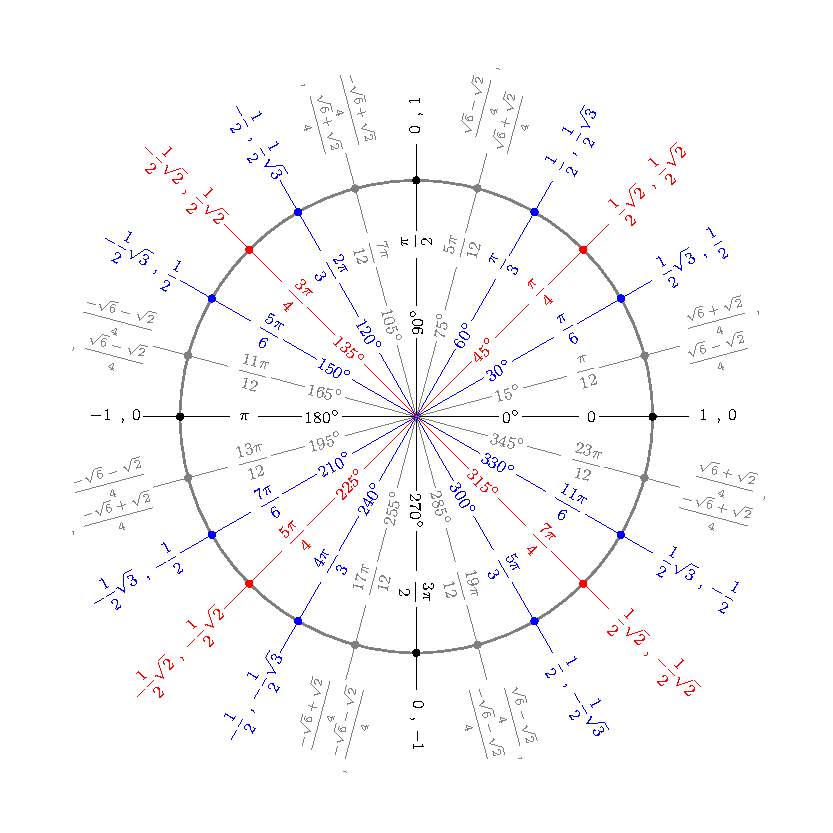
\includegraphics[width=\linewidth]{content/figures/einheitskreis_15}
\end{minipage}


\end{document}
